\documentclass{article}
\usepackage{multicol}
\usepackage{listings}
\usepackage[margin=1in]{geometry}
\usepackage{graphicx}
\usepackage{float}
\usepackage{subcaption}
\newcommand*{\Scale}[2][4]{\scalebox{#1}{$#2$}}
\newcommand*{\Resize}[2]{\resizebox{#1}{!}{$#2$}}
\graphicspath{ {./Figures/} }

\begin{document}

\section{Objectives}
\indent
The objective for this lab is to construct a sequence of shaped pulses and examine the role of pulse shape on intersymbol interference and the effect of noise.

\noindent
During this lab we will look at 4 difference types of line code:
  \begin{itemize}
    \item Polar
    \item On-Off
    \item Bipolar
    \item Duobinary
  \end{itemize}

\section{Procedure}

\subsection{Pulse Types}
During this lab we will be using a variety of pulse shapes. Below are the different pulse shapes that I used.

\subsubsection{Raised Cosine Pulse}
\begin{figure}[H]
  \begin{center}
    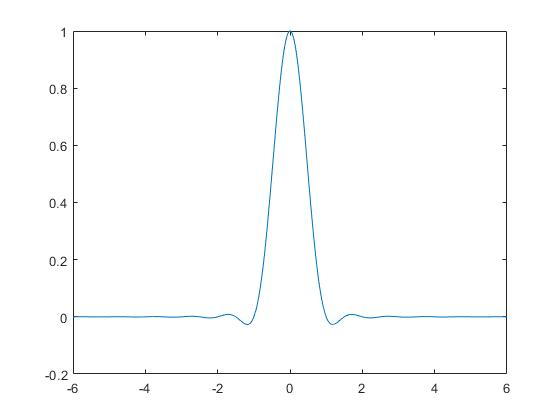
\includegraphics[width = 0.4\linewidth]{Raised_Cosine_Pulse.jpg}
    \caption{Raised Cosine Pulse}
    \label{fig:Raised_Cosine_Pulse}
  \end{center}
\end{figure}
\subsubsection{Triangle Pulse}
\begin{figure}[H]
  \begin{center}
    \begin{subfigure}[b]{0.4\linewidth}
      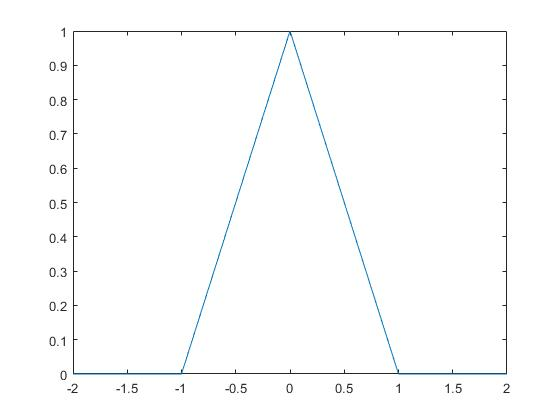
\includegraphics[width = \linewidth]{Tri_Half.jpg}
      \caption{Triangular Half Width Pulse}
    \end{subfigure}
    \begin{subfigure}[b]{0.4\linewidth}
      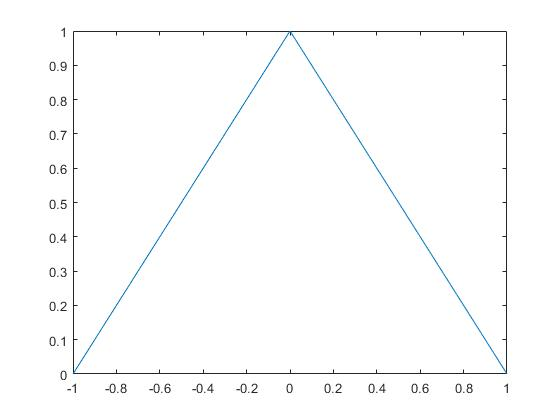
\includegraphics[width = \linewidth]{Tri_Full.jpg}
      \caption{Triangular Full Width Pulse}
    \end{subfigure}
    \caption{Triangular Pulse}
    \label{fig:Tri}
  \end{center}
\end{figure}
\subsubsection{Rectangle Half Width}
\begin{figure}[H]
  \begin{center}
    \begin{subfigure}[b]{0.4\linewidth}
      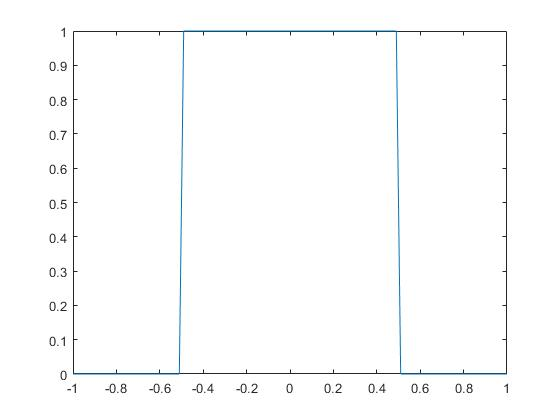
\includegraphics[width = \linewidth]{Rect_Half.jpg}
      \caption{Rectangular Half Width Pulse}
    \end{subfigure}
    \begin{subfigure}[b]{0.4\linewidth}
      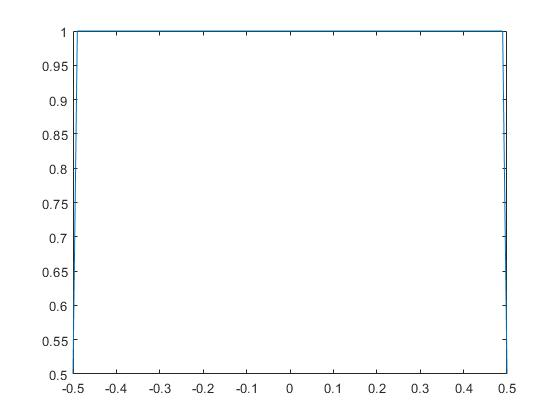
\includegraphics[width = \linewidth]{Rect_Full.jpg}
      \caption{Rectangular Full Width Pulse}
    \end{subfigure}
    \caption{Triangular Pulse}
    \label{fig:Rect}
  \end{center}
\end{figure}
\subsubsection{Sinc}
\begin{figure}[H]
  \begin{center}
    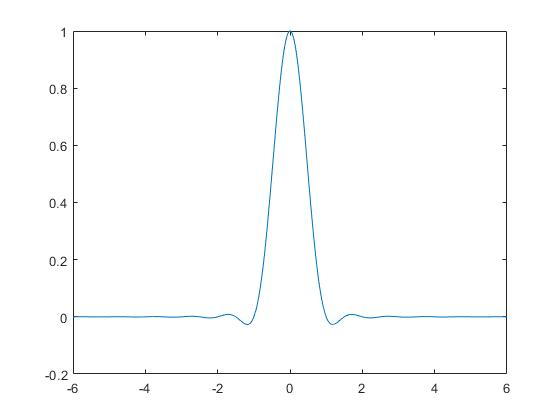
\includegraphics[width = \linewidth]{Raised_Cosine_Pulse.jpg}
    \caption{Raised Cosine Pulse}
    \label{fig:Sinc-Pulse}
  \end{center}
\end{figure}
\subsubsection{Sinc Squared}
\begin{figure}[H]
  \begin{center}
    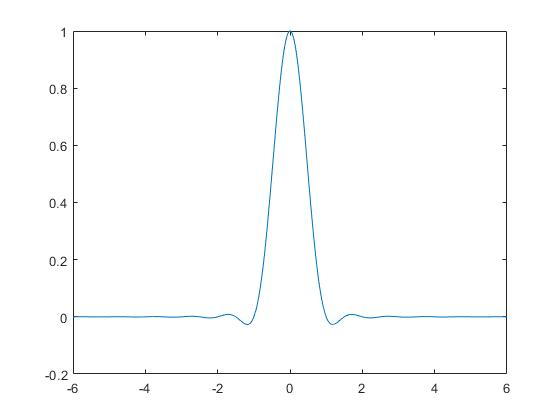
\includegraphics[width = \linewidth]{Raised_Cosine_Pulse.jpg}
    \caption{Raised Cosine Pulse}
    \label{fig:Sinc-Squared}
  \end{center}
\end{figure}
\subsection{Sin Pulse}
\begin{figure}[H]
  \begin{center}
    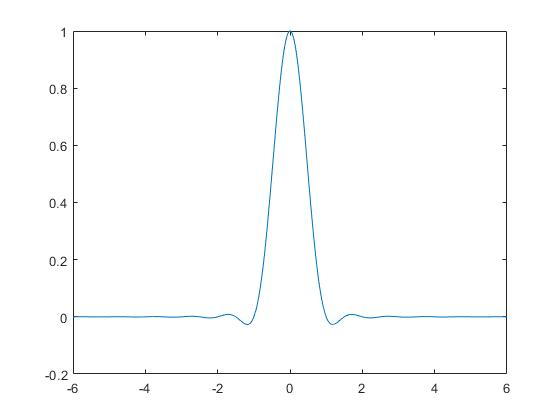
\includegraphics[width = \linewidth]{Raised_Cosine_Pulse.jpg}
    \caption{Raised Cosine Pulse}
    \label{fig:Sin-Pulse}
  \end{center}
\end{figure}

\section{Results}

\subsection{On-Off}
\begin{figure}[H]
  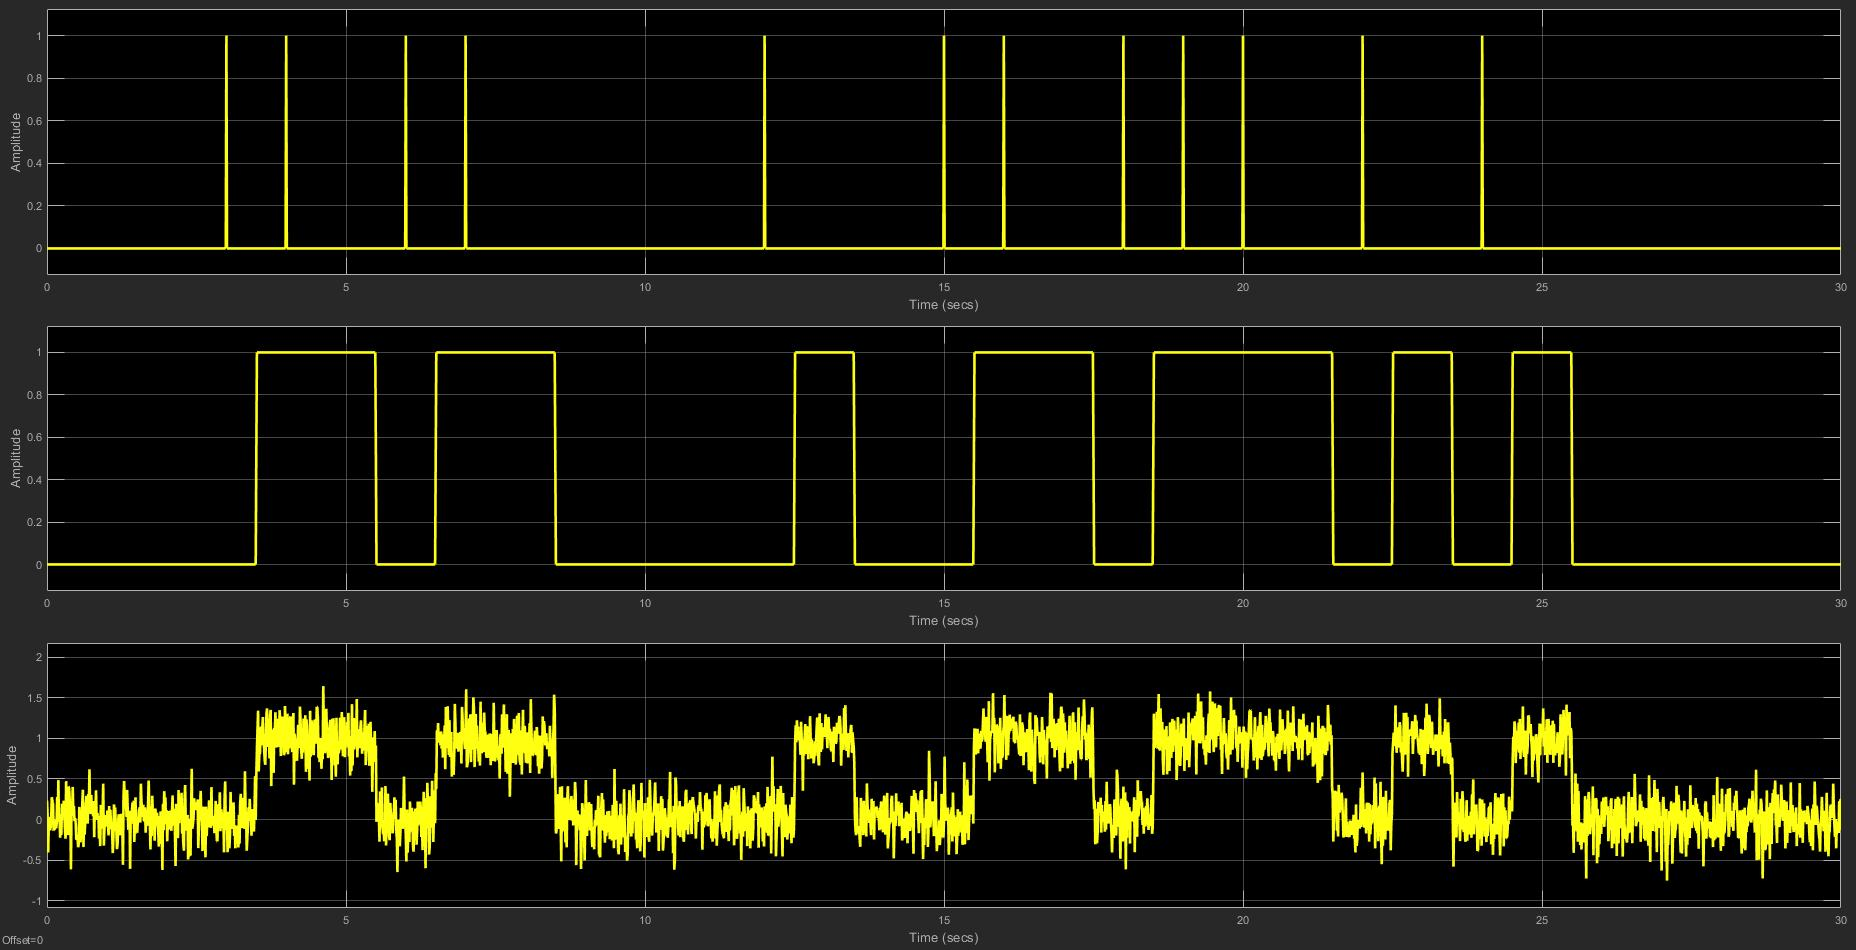
\includegraphics[width = \linewidth]{On_Off.jpg}
  \caption{On-Off line Code Results}
  \label{fig:on-Off}
\end{figure}
This fugre is a result of the on-off line code.The firse plot is of the binary
that was generated. The second plot is using the Rectangular Full Width shaped pulse
The third plot is of the recieved signal with noise on the channel. In Figure \ref{fig:on-Off}.

\subsection{Polar}

\subsection{Bipolar}

\subsection{Duobinary}



\end{document}
